The \textbf{Maximum Matching Problem} stands as one of the most fundamental challenges in graph theory, with critical relevance to solving complex, real-world problems. Finding a maximum matching extends beyond theoretical interest; it has practical applications in areas such as job assignments, resource allocation, and network connectivity. For example, consider matching a set \( M \) of machines with a set \( T \) of tasks to be performed at the same time. An edge \((u, v) \in E\) means that a machine \( u \in M \) can perform a task \( v \in T \). A maximum matching provides work for as many machines as possible. In this context, an optimal matching ensures that no machine is left idle if there are tasks available, and no task is left incomplete if a machine is capable of performing it. This framework can also be applied to other areas, such as assigning employees to projects or distributing resources efficiently across a network.



The formal definition of the Maximum Matching Problem can be stated as follows:

\begin{center}
    \begin{tabular}{rl} % Right (r) and left (l) alignment
        \textbf{Input}: & Let \(V\) be a set, \(d \geq 2\) be an integer, and \(G = \langle V_d, E \subseteq V_d \rangle\) be a \(d\)-partite graph. \\
        \\
        \textbf{Output}: & \begin{minipage}[t]{0.7\textwidth}
        A maximum matching \(M\) of \(G\), that is, the largest set \(M \subseteq E\) such that for each pair of different edges \(e_1, e_2 \in M\), the vertices in the corresponding positions of \(e_1\) and \(e_2\) in the edges are distinct.
        \end{minipage}
    \end{tabular}
\end{center}

A maximum matching in a graph is defined as a matching that encompasses the largest possible number of edges, ensuring that no other matching can contain more edges than this optimal set \cite{cormen2009introduction}. The largest matching can be at most \( |V| = n \), where \( V \) is the set of vertices in the graph. It is important to note that for all vertices \( v \in V \), at most one edge of \( M \) is incident on \( v \). This property ensures that the matching does not have any duplicate connections, maintaining a one-to-one correspondence between matched vertices. 

To illustrate this concept, consider the bipartite graph depicted in Figure \ref{fig:max_match_bipartite_graph}. In this graph, the vertices are divided into two distinct sets, and edges connect vertices from one set to the other. This straightforward example captures the essence of the maximum matching problem, showcasing the interplay between structure and optimization in graph theory.
\newpage

\begin{figure}[ht]
\centering
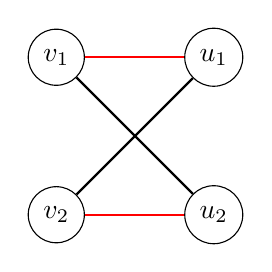
\begin{tikzpicture}[scale=1, transform shape]
    % Nodes
    \node[draw, circle] (v1) at (0,2) {$v_1$};
    \node[draw, circle] (v2) at (0,0) {$v_2$};
    \node[draw, circle] (u1) at (2,2) {$u_1$};
    \node[draw, circle] (u2) at (2,0) {$u_2$};
    
    % Edges
    \draw[red, thick] (v1) -- (u1);   % Matching edge
    \draw[red, thick] (v2) -- (u2);   % Matching edge
    \draw[black, thick] (v1) -- (u2); % Non-matching edge
    \draw[black, thick] (v2) -- (u1); % Non-matching edge
\end{tikzpicture}
\caption{A bipartite graph with maximum matching highlighted in red.}
\label{fig:max_match_bipartite_graph}
\end{figure}


The matching \( M \) for this bipartite graph is defined as:
\[
M = \{ (v_1, u_1), (v_2, u_2) \}
\]



The complexity of the Maximum Matching Problem can vary significantly depending on the type of graph being used. In the case of a \(d\)-partite graph, where the vertex set \(V\) is partitioned into \(d\) subsets, the goal is to find a maximum matching \(M \subseteq E\) such that no two edges in \(M\) share any vertices from the same subset. As \(d\) increases, particularly for \(d \geq 3\), the problem becomes NP-complete, meaning that exact algorithms become infeasible for large instances.

For example, in a hypergraph graph, the challenge lies in effectively navigating the combinations of edges while ensuring distinctness among the vertices involved in the matched pairs. Consider the example shown in Figure \ref{fig:tripartite_graph}.

\begin{figure}[t]
\centering
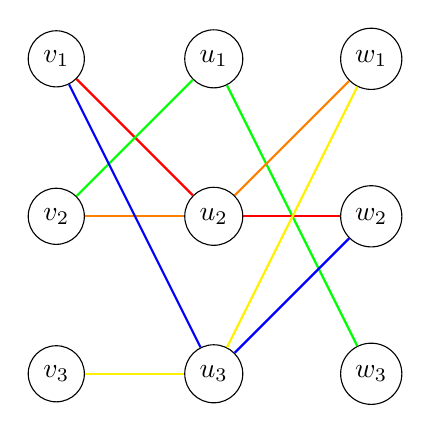
\begin{tikzpicture}[scale=1, transform shape]
    % Nodes
    \node[draw, circle] (v1) at (0,4) {$v_1$};
    \node[draw, circle] (v2) at (0,2) {$v_2$};
    \node[draw, circle] (v3) at (0,0) {$v_3$};
    \node[draw, circle] (u1) at (2,4) {$u_1$};
    \node[draw, circle] (u2) at (2,2) {$u_2$};
    \node[draw, circle] (u3) at (2,0) {$u_3$};
    \node[draw, circle] (w1) at (4,4) {$w_1$};
    \node[draw, circle] (w2) at (4,2) {$w_2$};
    \node[draw, circle] (w3) at (4,0) {$w_3$};
    % Edges
    \draw[red, thick] (v1) -- (u2);   % Matching edge
    \draw[orange, thick] (v2) -- (u2);
    \draw[yellow, thick] (v3) -- (u3); % Matching edge
    \draw[green, thick] (v2) -- (u1);  % Matching edge
    \draw[blue, thick] (v1) -- (u3);   % Non-matching edge
    \draw[green, thick] (u1) -- (w3);  % Non-matching edge
    \draw[orange, thick] (u2) -- (w1); % Matching edge
    \draw[red, thick] (u2) -- (w2);    % Non-matching edge
    \draw[yellow, thick] (u3) -- (w1); % Non-matching edge
    \draw[blue, thick] (u3) -- (w2);   % Non-matching edge
\end{tikzpicture}
\caption{A hypergraph with maximum matching.}
\label{fig:tripartite_graph}
\end{figure}

The maximum matching \( M \) for this tripartite graph is defined as:
\[M = \{ (v_1, u_2, w_2), (v_2, u_1, w_3), (v_3, u_3, w_1) \}\]

This matching connects the vertices across the three sets while ensuring that no two edges share a vertex, thereby maximizing the total number of matched pairs.



The Maximum Matching Problem serves as a critical foundation for understanding complex graph interactions and their applications, providing a gateway into more advanced concepts and algorithms in the realm of graph theory. As mentioned, when \(d \geq 3\), the problem becomes NP-complete, meaning that finding an exact solution is computationally infeasible for large graphs. This motivates the exploration of approximation algorithms and heuristic approaches in practical scenarios.


